\documentclass[a4paper,10pt, nofootinbib]{article}
\usepackage[width=15.5cm, left=3cm, top=2.5cm, right=1cm, left=2cm, height= 24.5cm]{geometry}
\usepackage[spanish]{babel}
\usepackage[utf8]{inputenc}
\usepackage[T1]{fontenc}
\usepackage{xspace}
\usepackage{xargs}
\usepackage{ifthen}
\usepackage{caratula}
\usepackage{fancyhdr}
\usepackage[bottom]{footmisc}
\usepackage{modulos}
\usepackage{algorithm}
\usepackage[noend]{algpseudocode}
\usepackage{float}
\usepackage{amsmath}

\usepackage{graphicx}
\graphicspath{ {images/} }

\newcommand{\moduloNombre}[1]{\textbf{#1}}


\let\NombreFuncion=\textsc
\let\TipoVariable=\texttt
\let\ModificadorArgumento=\textbf
\newcommand{\res}{$res$\xspace}
\newcommand{\tab}{\hspace*{7mm}}

\newcommand{\Ogr}{\mathcal{O}}


\newcommand{\footnoteMio}[2]{\textsuperscript{#1} \lfoot{\footnotesize \parbox{16cm}{\textsuperscript{#1}#2}}}

\newcommandx{\TipoFuncion}[3]{%
  \NombreFuncion{#1}(#2) \ifx#3\empty\else $\to$ \res\,: \TipoVariable{#3}\fi%
}
\newcommand{\In}[2]{\ModificadorArgumento{in} \ensuremath{#1}\,: \TipoVariable{#2}\xspace}
\newcommand{\Out}[2]{\ModificadorArgumento{out} \ensuremath{#1}\,: \TipoVariable{#2}\xspace}
\newcommand{\Inout}[2]{\ModificadorArgumento{in/out} \ensuremath{#1}\,: \TipoVariable{#2}\xspace}
\newcommand{\Aplicar}[2]{\NombreFuncion{#1}(#2)}

\newcommand{\Titulo}[1]{
  \vspace*{1ex}\par\noindent\textbf{\large #1}\par
}
\newcommand{\DRef}{\ensuremath{\rightarrow}}

%%Información para la carátula
\materia{Organizacion del Computador II}

\titulo{\LARGE Trabajo Práctico N2}

\grupo{Grupo rafrani}
\integrante{Ruiz Ramirez, Emanuel}{343/15}{ema.capo2009@hotmail.com}
\integrante{Serio, Franco}{215/15}{francoagustinserio@gmail.com }
\integrante{Soberon, Nicolás}{641/10}{nico.soberon@gmail.com}

\def\cuatrimestre{1}

%%fancyhdr
\pagestyle{fancy} 
\thispagestyle{fancy}
\addtolength{\headheight}{1pt}
\lhead{Algoritmos y Estructuras de Datos II: TP2}
\rhead{$2^{\mathrm{do}}$ cuatrimestre de 2016}
\cfoot{\thepage\ / 30}
\renewcommand{\footrulewidth}{0.4pt}



\setlength{\parskip}{0.8em}


\begin{document}
\maketitle

\tableofcontents
\clearpage

\thispagestyle{empty}


\clearpage

\section{Introducci\'on}
Este Trabajo Pr\'actico se basa en utilizar el modelo de procesamiento SIMD (Single Instruction Multiple Data) por medio del uso de instrucciones SSE (Streaming SIMD Extensions), para poder desarrollar distintos metodos para 'Navier Stokes' y asi poder evaluar el rendimiento de las mismas.
Algunas de las ventajas de usar las instrucciones SSE:
Ejecutar de manera paralela (simultaneamente) la misma instrucci\'on sobre distintos datos.
Utilizar los registros XMM, los cuales nos sirven para operar con datos empaquetados y de punto flotante.
Reducir los accesos a memoria, ya que podemos guardar mas datos en registros y con una sola instrucci\'on mover 128 bits a memoria.

Se implementaron los siguientes metodos en Assembler:

\begin{itemize}
\item \textbf{solver\_lin\_solve} : Se encarga de calcular la difusion del fluido a modelar.
\item \textbf{solver\_set\_bnd}: Calcula los valores para los casos borde de las matrices.
\item \textbf{solver\_project}: Proyecta los nuevos valores en la matriz de velocidad
\end{itemize}



\clearpage

\section{Desarrollo}
Vamos a trabajar con matrices. Estas matrices de velocidad son la representaci\'on discreta del campo vectorial asociado simplificado al tomar un vector representante de la grilla obtenida al dividir el espacio en celdas de tama\~o fijo. En estas matrices agregamos una columna y una fila a cada lado de nuestra grilla para simplificar el trabajo sobre los bordes.
Al recorrer la matriz, vamos a poder acceder a 4 celdas a la vez. De esta manera podemos aprovechar el modelo SIMD, para poder operar con estos datos juntos, y asi realizar menos iteraciones.

\subsection{solver\_lin\_solve}
La manera en la que opera una iteracion del ciclo mas superficial de solver$\_$lin$\_$solve es:
\begin{itemize}
\item Primero guardo en edx N+2, es decir la cantidad de elementos de una fila.
\item En el for i, se va a realizar las modificaciones para cuatro columnas contiguas empezando desde l primera y avanzando de a cuatro columnas.
\item Al comienzo de for i, rax quiero que apunte a la posicion (i,1) de la matriz x y r8 apunta a la misma posicion pero en la matriz x0. Tambien me traigo a xmm4 el bloque de 4 floats contiguos que comienza en (i,0).
\item En el for j, se va a realizar las modificaciones para un bloque de cuatro floats contiguos que comienzan en la posicion (i,j) y se va a ir avanzando de a una fila
\item Dentro del for j, tanto rax y r8 van a apuntar a la pos (i,j) de sus respectivas matrices. Y hago los siguientes accesos a memoria, en xmm2 traigo los cuatro floats contiguos que comienzan en (i,j+1) de x, en xmm3 traigo a los que comienzan en (i+1,j) de x, en xmm5 traigo a los que comienzan en (i-1,j) de x y en xmm6 traigo a los que comienzan en (i,j) de x0. En xmm4 estaria el bloque que comienza en (i,j-1) de x  que lo tengo  de la iteracion anterior, si es que no estoy en la primera iteracion, pero en caso de estarlo traigo a los cuatro floats de (i,0) de x.
\item Usando las operaciones de SIMD correspondientes hago que a cada float de xmm0 cuyo valor es 'a' multiplique a cada float de xmm2, xmm3 y xmm4. Tambien  cada float de xmm1 cuyo valor es 'c' divide a cada float de xmm2, xmm3, xmm4 y xmm6.
\item Para modificar el contenido del bloque de cuatro floats que comienzan en (i,j) de x, a xmm6 le sumo xmm2 y xmm3, ya que los floats de xmm2 y xmm3 son los valores de matriz x aun no modificados. Tambien le sumo xmm4, ya que los floats de xmm4 son los valores de la matriz x ya modificados o de la fila 0 en caso de ser la primera iteracion. Por ultimo, le sumo a cada float de xmm6 su respectivo valor de la izquierda ya modificado. Para hacer esto, armo el valor de la izquierda, lo multiplico por 'a' y divido por 'c' para despues sumarlo en la posicion correspondiente. Entonces lo obtenido en xmm6 lo guardo en lo apuntado por rax y en xmm4 para usarlo en la siguiente iteracion. 
\item Antes de terminar una iteracion de j, actualizo rax y r8 moviendolos N+2 floats. La idea es seguir en la siguiente fila. 
\item Antes de terminar una iteracion de i, actualizo rcx para que valga N+2, asi puedo armar rax en la siguiente iteracion. La idea es seguir con las siguientes 4 columnas.
\item Hago un llamado a solver$\_$set$\_$bnd, pasandole los parametros apropiados. Despues del llamado reconstruyo xmm0 para que tenga cuatro float 'a' y xmm1 posea cuatros float 'c'.
\item Si bien no corresponde a una iteracion, aclaro que uso los 5 registros que preservan su valor segun la convencion guardando 5 de los 6 parametros. El parametro faltante b y la variable local k las apilo en el stack(apilo primero b y despues k).
\end{itemize}

\subsection{solver\_set\_bnd}
Solver$\_$set$\_$bnd se implementó de la siguiente manera:
\begin{itemize}
\item Se guarda antes del ciclo los valores que hay en rdx y en rdi que son el puntero a x y el puntero a solver respectivamente. De este ultimo se saca el N, que es el tamaño de la matriz.
\item En r9 se guarda N+2. Se divide el N por 4 ya que es la cantidad de veces que va a iterar el ciclo.
\item se guarda el b en r13 y se testea que es (0, 1 o 2).
\item Si b es 1 o 0 se va a la parte llamada ciclo1 y si es 2 al ciclo2. El ciclo1 y ciclo2 son los ciclos que tratan la primera y ultima fila de los bordes, tanto si es 2, como 1 o 0.
\item Ciclo1 levanta 4 floats de memoria de la fila 1, y los pone en memoria en la fila 0. Luego va a la anteultima fila, levanta 4 y avanza a la ultima fila y los pone en memoria. Luego reestablezco el puntero y avanzo 16 bytes (4 floats) que son los que hice el la fila 0 y en la fila N+1. Idem para ciclo2 con la diferencia que antes de meterlos en memoria multiplico por xmm4 que es una mascara de -1.0, para pasar todo a negativos.
\item Luego se pasa a hacer la primera columna y por ultimo la ultima columna. Todo esto, como no se trabaja en un espacio continuo de memoria, no tiene ventajas utilizar SIMD por lo que aparte de utilizar xmm0 se utilizan los registros convencionales.
\item Si b es 0 o 2 se corre el finCiclo2 y si es 1 finCiclo1.
\item Los ciclos de primera columna son iguales con excepción del caso de b = 1 donde con la máscara xmm4 se hace negativo el resultado antes de insertarlo en memoria.
\item Idem para ultimaColumna de cada ciclo. Tanto primeraColumnaciclo1 como primeraColumnaCiclo2 y ultimaColumnaCiclo1 y ultimaColumnaCiclo2 usan r15 como puntero y r13 como contador. Todos estos ciclos van de 1 hasta que r13 < \ N + 1.
\item Por último ambos ciclos van a la etiqueta .fin, donde se procesa los lugares de los vértices de la matriz.
\item Los primeros sumandos se guardan en xmm0 y los segundos en xmm1.
\item La posicion de cada vértice en cada xmm es en el orden que están en el código de C. Por ejemplo, en los primeros 32 bits de xmm0 esta x[IX(1,0)] y de xmm1 x[IX(0,1)] para poder hacer el x[IX(0,0)].

\item Se suman xmm0 y xmm1

\item Luego se multiplica xmm0 por xmm11 que es una máscara con floats de 0.5

\item Finalmente insertamos xmm0 en memoria.

\item Reorganizamos el stack y retornamos.

\end{itemize}

\subsection{solver\_project}
En cuanto al desarrollo de solver\_project, tuvimos q aplicar una f\'ormula a cada celda de la matriz, luego llamar solver\_set\_bnd y solver\_lin\_solve, y luego volver a procesar las celdas de la matriz.
El m\'etodo funciona de la siguiente manera:

\begin{itemize}
\item El algoritmo cuenta con un ciclo incial, llamado a funciones auxiliares, otro ciclo, y otro llamado a funciones auxiliares.
\item Para recorrer toda la matriz, vamos a realizar dos ciclos, uno dentro de otro, que van a ir desde 1 hasta N + 1, de esta manera no caemos en un caso que no se pueda resolver, ya que los bordes van a ser seteados cuando se llame a $solver_set_bnd$.
\item Vamos a procesar 4 celdas por iteraci\'on del ciclo, de esta manera, podemos procesar m\'ultiples datos en cada iteraci\'on.
\item Empezamos guardandonos m\'ascaras, que contienen $|N|N|N|N|$ y $|-0.5f|-0.5f|-0.5f|-0.5f|$, para poder realizar los c\'alculos necesarios.
\item Luego, pasamos al primer ciclo, comenzamos por traer 4 celdas de source al comienzo del ciclo.
\item Para operar con las celdas en posiciones $j+1$ y $j-1$, vamos a traernos en cada iteraci\'on las 4 celdas actuales, las 4 celdas que se encuentran en la fila anterior, restando una fila al contador de filas, arriba de las actuales y las 4 celdas de la fila siguiente, sumando una fila al contador de las filas, que se encuentran debajo de las actuales.
\item De esta manera podemos realizar el c\'omputo $solver->u[IX(i+1,j)] - solver->u[IX(i-1,j)]$
\item Luego, vamos a traernos las 4 celdas anteriores de la misma fila y las 4 celdas siguientes de la misma fila.
\item Utilizando SHIFTS vamos a acomodar los dos registros XMM de manera tal que podamos realizar la resta correspondiente, y obtener el valor de $j+1$ - $j-1$ para las cuatro posiciones que estamos mirando.
\item De esta manera podemos computar $solver->v[IX(i,j+1)] - solver->v[IX(i,j-1)]$
\item Luego, restamos estos dos valores calculados anteriormente, para poder obtener $(solver->u[IX(i+1,j)] - solver->u[IX(i-1,j)] + solver->v[IX(i,j+1)] - solver->v[IX(i,j-1)])$
\item Luego, utilizando las m\'ascaras que guardamos al principio, utilizando multiplicaciones y divisiones, podemos calcular $div[IX(i,j)] = - 0.5f * (solver->u[IX(i+1,j)] - solver->u[IX(i-1,j)] + solver->v[IX(i,j+1)] - solver->v[IX(i,j-1)]) / solver->N$.
\item A parte de realizar la asignaci\'on anterior, vamos a asignar ceros para realizar $p[IX(i,j)] = 0;$
\item Luego, vamos a tener los llamados a $solver_set_bnd ( solver, 0, div )$, $solver_set_bnd ( solver, 0, p )$ y $solver_lin_solve ( solver, 0, p, div, 1, 4 )$.
\item Luego, vamos a tener el segundo ciclo, este va a estar construido de la misma manera que el anterior, y el procesamiento de datos se va a realizar de la misma manera, la \'unica diferencia es que las operaciones se van a realizar trayendo los datos de otro puntero. Pero el funcionamiento y la manera de recorrerlo, es igual al anterior.
\item Por \'ultimo vamos a realizar los llamados correspondientes a $solver_set_bnd ( solver, 1, solver->u )$ y $solver_set_bnd ( solver, 2, solver->v )$
\end{itemize}

De esta manera podemos aplicar el modelo SIMD a nuestro m\'etodo. Aprovechando poder trabajar con m\'ultiples datos a la vez, nos vamos a ahorrar operaciones, lo que implica un menor tiempo de c\'omputo, y una mejor performance de nuestro algoritmo.

 

\clearpage

\section{Resultados}
\graphicspath{{./img/}}

Nuestra Hipotesis a la hora de experimentar, es que, utilizar el modelo SIMD con operaciones SSE, nos da una mayor performance a la hora de desarrollar nuestros algoritmos. El hecho de poder procesar varios datos a la misma vez, nos permite ahorrarnos tiempo de ejecucion y cantidad de iteraciones en nuestros algoritmos.
Realizamos distintas corridas de nuestro codigo, tanto en ASM, como en C con las correspondientes optimizaciones que nos permite el compilador. De esta manera pudimos respaldar nuestra hipotesis con resultados concretos.

\subsection{solver\_lin\_solve}

El objetivo a alcanzar fue que la implementacion de solver$\_$lin$\_$solve en asm tarda menos que alguna de las implementaciones de c en O, O2 u O3. Para ello se hizo un experimento en el cual para un nivel de optimizacion ejecuto 1000 veces la funcion en asm y en c para tres tamaños diferentes de matrices. Por cada llamado se le va a tomar el tiempo, es decir la cantidad de clocks que le toma en ejecutarse. Ademas para evitar por ejemplo que los clocks que le toma a la funcion en asm para la matriz de tamaño 256 sean altos en principio y luego bajen mucho, lo que se hace es llamar a la funcion de asm con un tamaño de matriz despues a la de c con un tamaño de matriz diferente e ir intercalando los llamados sucesivamente. 
El valor del parametro 'b' se lo dejo fijo porque no lo usa solver$\_$lin$\_$solve ya que se lo pasa a solver$\_$set$\_$bnd. El valor de 'a' y 'c' se los dejo fijos, ya que solo multiplican y dividen valores para modificar una de las matrices que se le pasan por parametreo a solver$\_$lin$\_$solve.
Para un tamaño de matriz en un fichero estaran los clocks que le toma ejecutar a la funcion de c en O0, abajo siguen los clocks de O2 y por ultimo estan los de O3. Los clocks que le toman a la funcion de asm se guarda de la misma forma que c.
  

\begin{figure}[h]
  \centering
    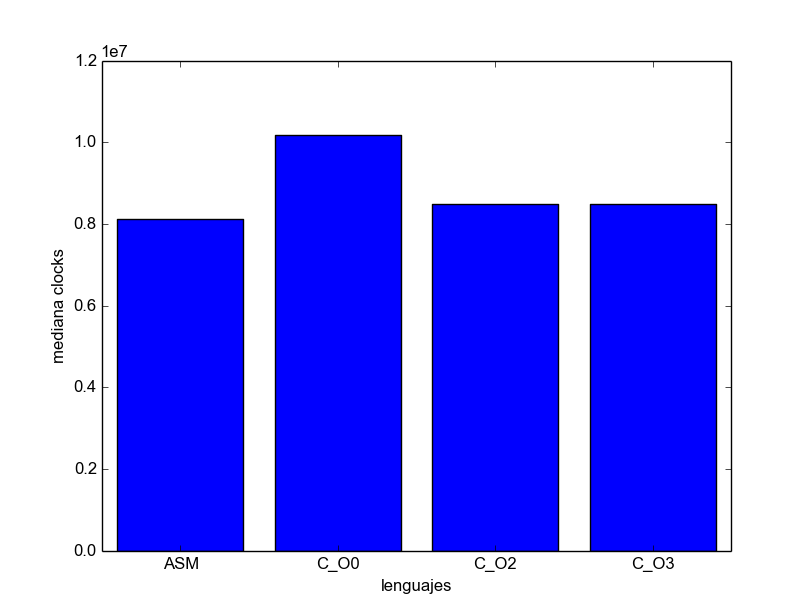
\includegraphics[width=.6\linewidth]{Matriz_128.png}
    \caption{Performance para Matriz 128x128}
    \label{fig:M128}
\end{figure}

\pagebreak

\begin{figure}[h]
  \centering
    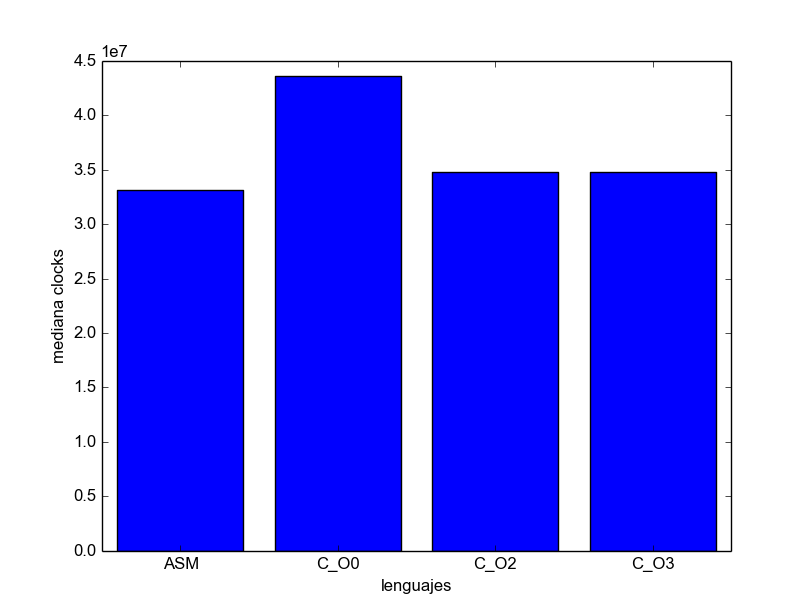
\includegraphics[width=.6\linewidth]{Matriz_256.png}
    \caption{Performance para Matriz 256x256}
    \label{fig:M256}
\end{figure}

\begin{figure}[h]
  \centering
    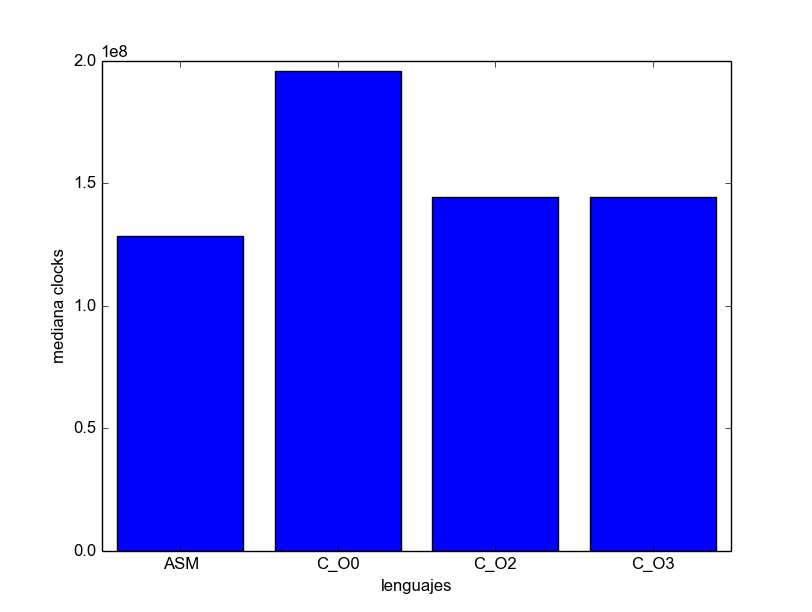
\includegraphics[width=.6\linewidth]{Matriz_512.png}
    \caption{Performance para Matriz 512x512}
    \label{fig:M512}
\end{figure}

\newpage

\subsection{solver\_set\_bnd}

En solver$\_$set$\_$bnd se hicieron 4 gráficos para comparar ASM y C con los distintos tamaños, que son iguales a los tamaños de las imágenes de la cátedra. El solver tiene 2 matrices de floats, que son las que utilizamos para hacer los experimentos en este caso. Si bien el $b$ se cambió en cada iteración para que el procesador no cachee los experimentos y tengamos tiempos medianamente razonables, no se graficó ya que no influye en el algoritmo.
Los pasos para los experimentos fueron los siguientes:
Por cada tamaño, en total 6, se hicieron 750 iteraciones. En cada iteración se corre un código diferente(ASM, C), con una matriz diferente (v o u) y con b diferente (0, 1, 2) a la iteración inmediata anterior. En todos los siguientes casos se utiliza la mediana como mediana.
Todo esto se vuelca en un csv, donde por python, con las bibliotecas NumPy y Matplotlib terminamos haciendo los gráficos. 

\begin{figure}[h]
  \centering
    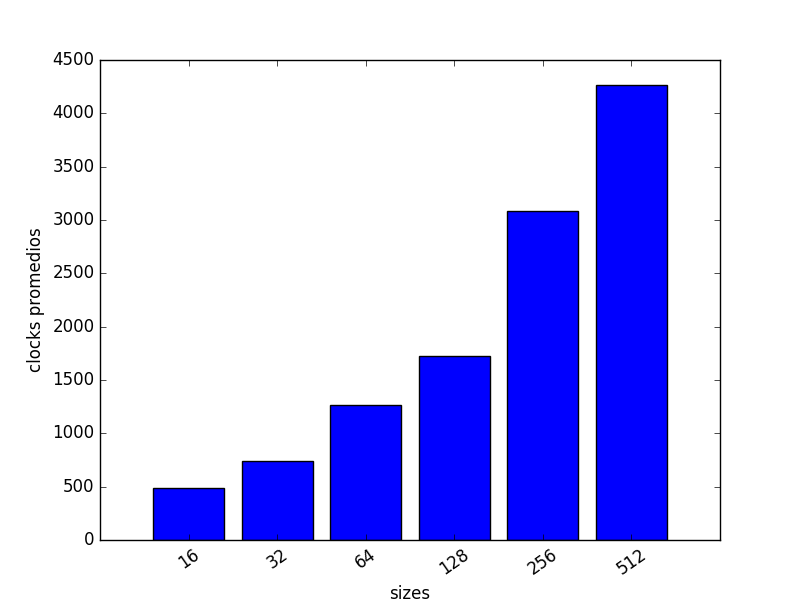
\includegraphics[width=.6\linewidth]{ClocksASMU.png}
    \caption{Código ASM con matriz U}
    \label{fig:ASMU}
\end{figure}

\pagebreak

\begin{figure}[h]
  \centering
    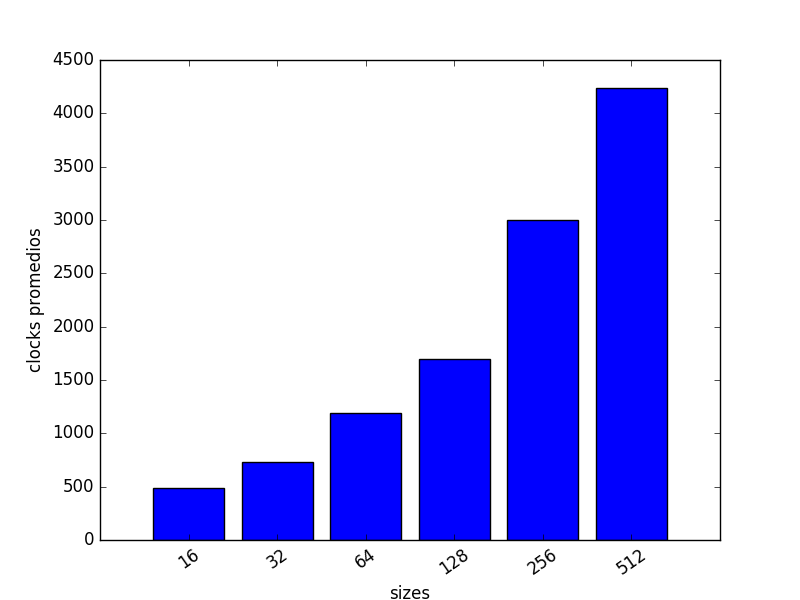
\includegraphics[width=.6\linewidth]{ClocksASMV.png}
    \caption{Código ASM con matriz V}
    \label{fig:ASMV}
  \centering
    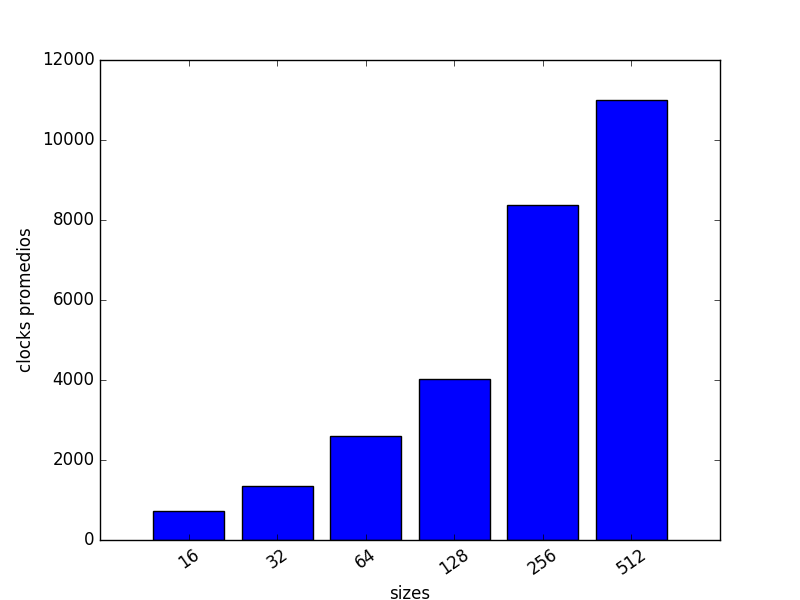
\includegraphics[width=.6\linewidth]{ClocksCU.png}
    \caption{Código C con matriz U}
    \label{fig:CU}
\end{figure}

\begin{figure}[h]
  \centering
    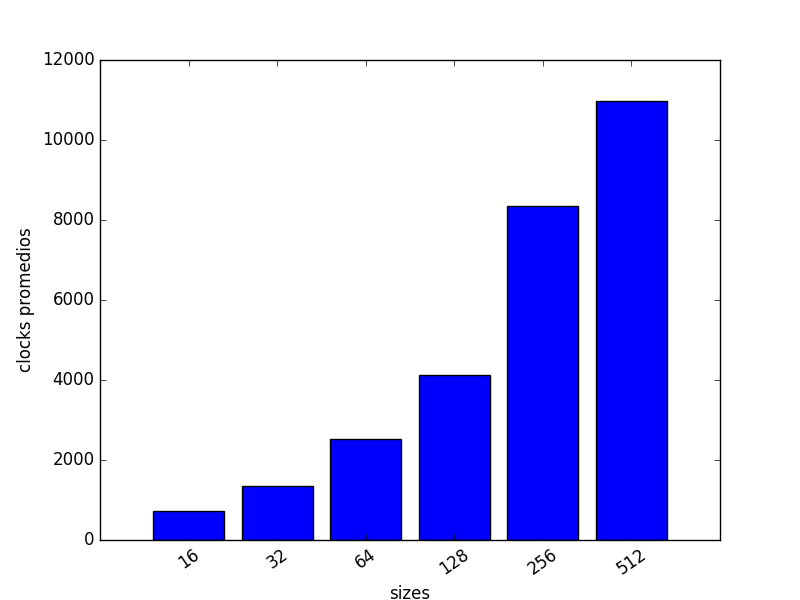
\includegraphics[width=.6\linewidth]{ClocksCV.png}
    \caption{Código C con matriz V}
    \label{fig:CV}
\end{figure}

\pagebreak

\subsection{solver\_project}

En $solver_project$ se realizaron 1000 ejecuciones de nuestro c\'odigo en ASM y nuestro c\'odigo en C, con las correspondientes optimizaciones O0, O2, O3. Las ejecuciones se realizaron para distintos tamaños de matrices.
Los tamaños que utilizamos fueron de 128x128, 256x256 y 512x512.
En cada ejecuci\'on, tomamos los tiempos de corrida del algoritmo, para poder utilizarlos para realiar gr\'aficos, para poder ver de manera mas clara cual es el rendimiento de nuestro c\'odigo en ASM comparado con el c\'odigo en C.
Las mediciones realizadas las almacenamos en un archivo csv, el cual utilizamos para realizar los gr\'aficos mencionados anteriormente.
Los gr\'aficos los realizamos utilizando codigo Python, con las bibliotecas Numpy y Matplotlib.
En los gr\'aficos, expuestos a continuaci\'on, podemos observar que nuestra hip\'otesis se cumple.
Es clara la superioridad de performance del codigo ASM con operaciones SIMD, a comparaci\'on de C.
Y lo que podemos ver es que por mas que utilicemos las distintas optimizaciones para compilar el c\'odigo C, igualmente el codigo ASM sigue siendo mas performante.

\begin{figure}[h]
  \centering
    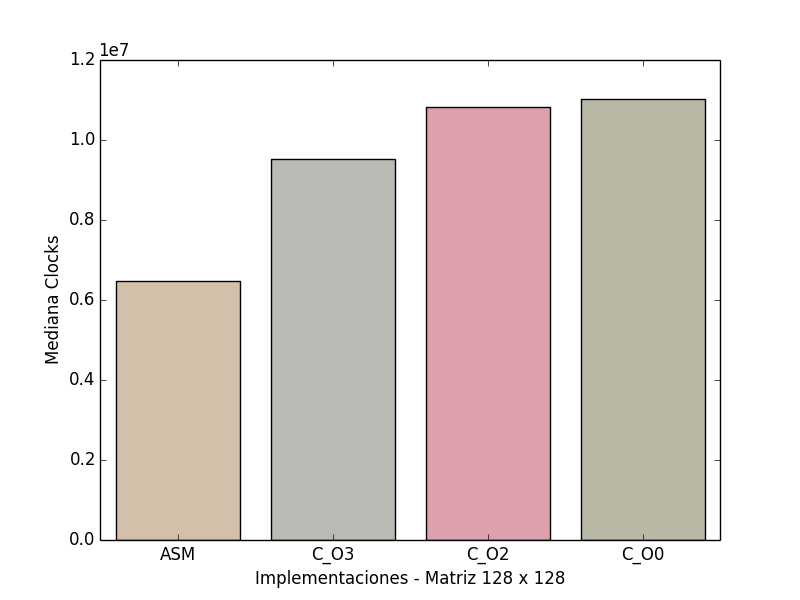
\includegraphics[width=.6\linewidth]{128x128.png}
    \caption{Tiempos para Matriz 128x128}
    \label{fig:M128}
\end{figure}

\pagebreak

\begin{figure}[h]
  \centering
    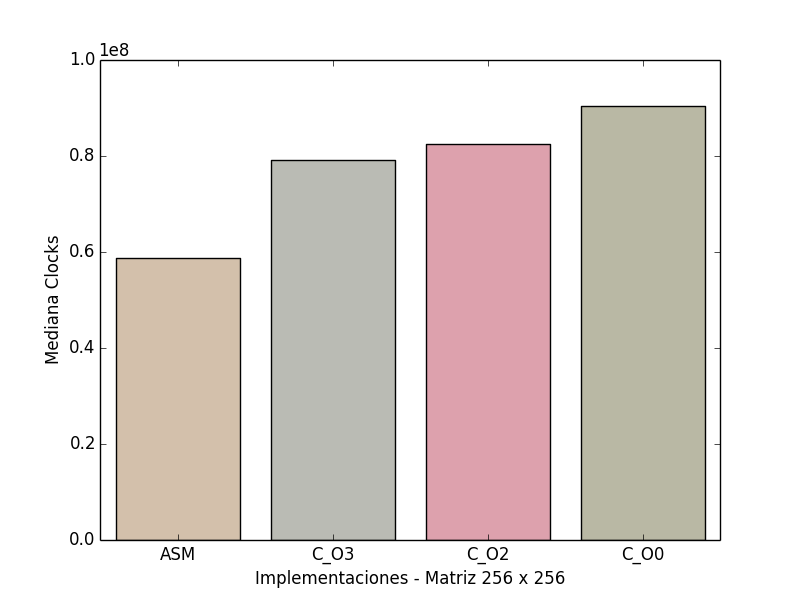
\includegraphics[width=.6\linewidth]{256x256.png}
    \caption{Tiempos para Matriz 256x256}
    \label{fig:M256}
\end{figure}

\begin{figure}[h]
  \centering
    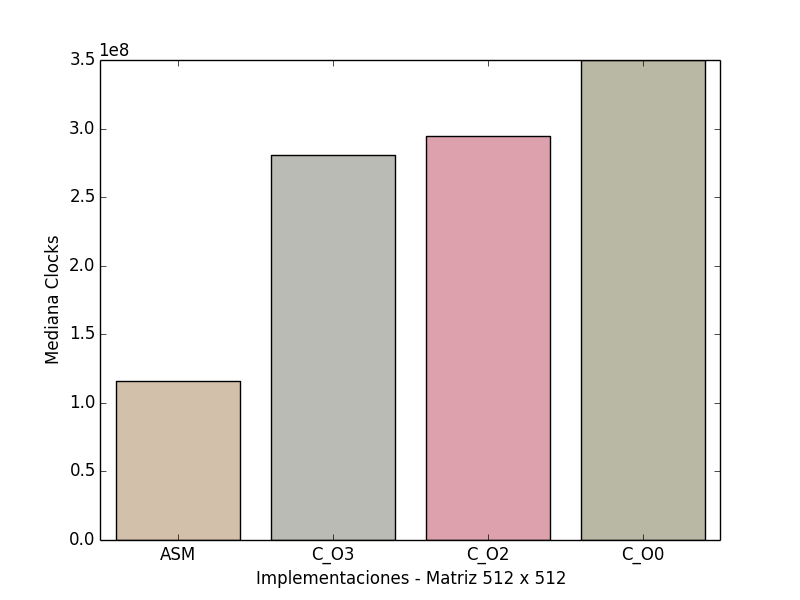
\includegraphics[width=.6\linewidth]{512x512.png}
    \caption{Tiempos para Matriz 512x512}
    \label{fig:M512}
\end{figure}


\clearpage

\section{Conclusi\'on}
\graphicspath{{./img/}}

\subsection{C vs ASM}

{\scshape\Large solver$\_$set$\_$bnd\par}

Como se puede apreciar en las figuras de la sección anterior, ASM tiene clocks mucho menores a las funciones en C en todos los tamaños si bien en los mas chicos (por ejemplo 16) las performances entre C y ASM son bastante equivalentes, como lo demuestra el gráfico de abajo. A su vez también vemos que la matriz U tarda en procesar mas ciclos de clock que la matriz V.

\begin{figure}[h]
  \centering
  	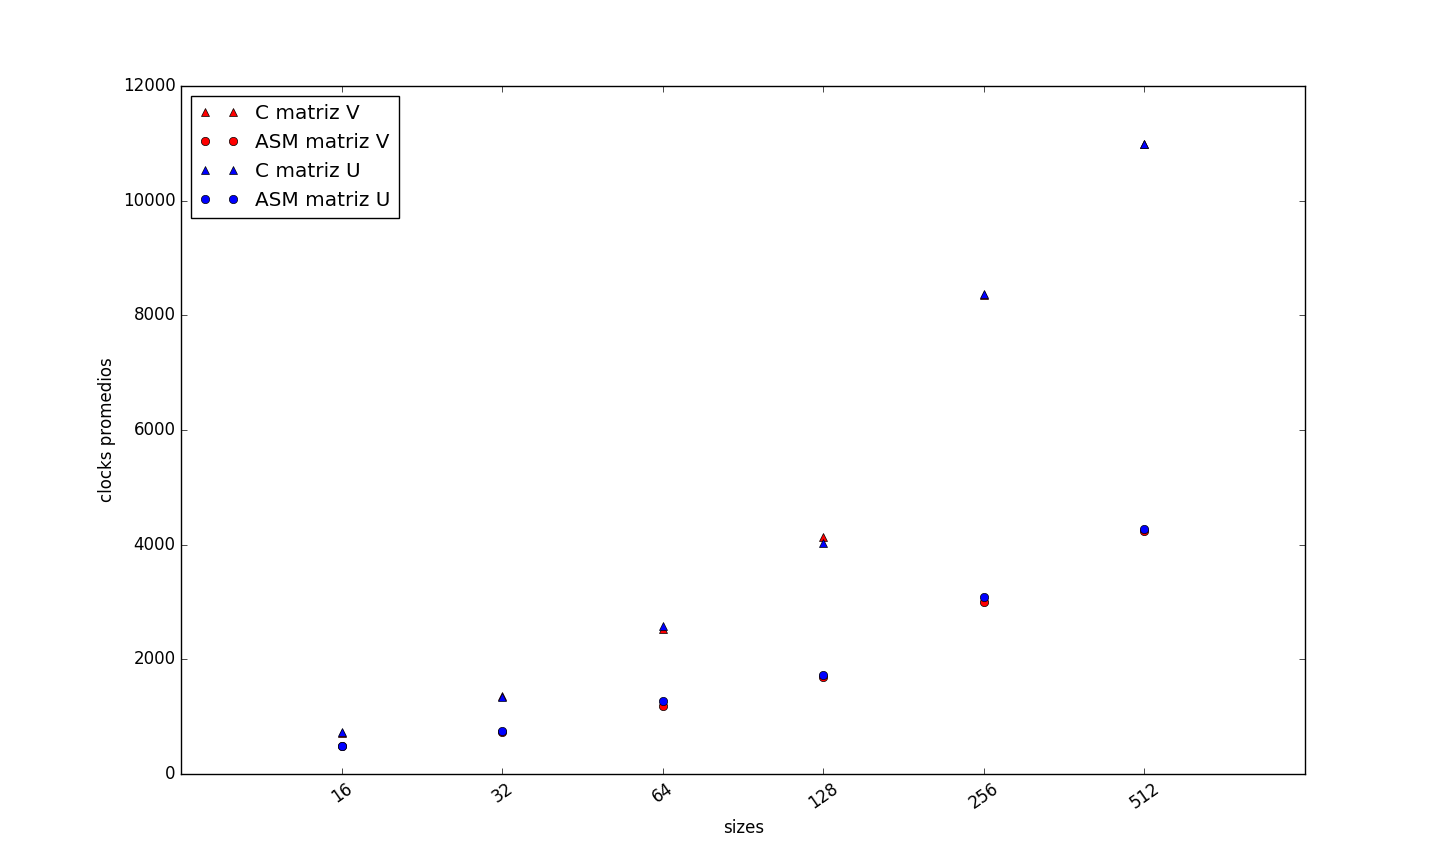
\includegraphics[width=.6\linewidth]{ClocksCYASM.png}
  	\caption{ASM VS C solver$\_$set$\_$bnd}
  	\label{fig:ASMU}
\end{figure}

A su vez, si en vez de 750 repeticiones se hicieran menos, los datos que se obtienen cada vez son mas proclives a errores. Concluimos que por la ley de los grandes números cuando tenemos una muestra menor se pueden producir varios errores en las experimentaciones como lo demuestra el siguiente gráfico con 200 iteraciones. Se pueden comparar fácilmente con los datos obtenidos y postulados en la sección Resultados.

\begin{figure}[h]
  \centering
  	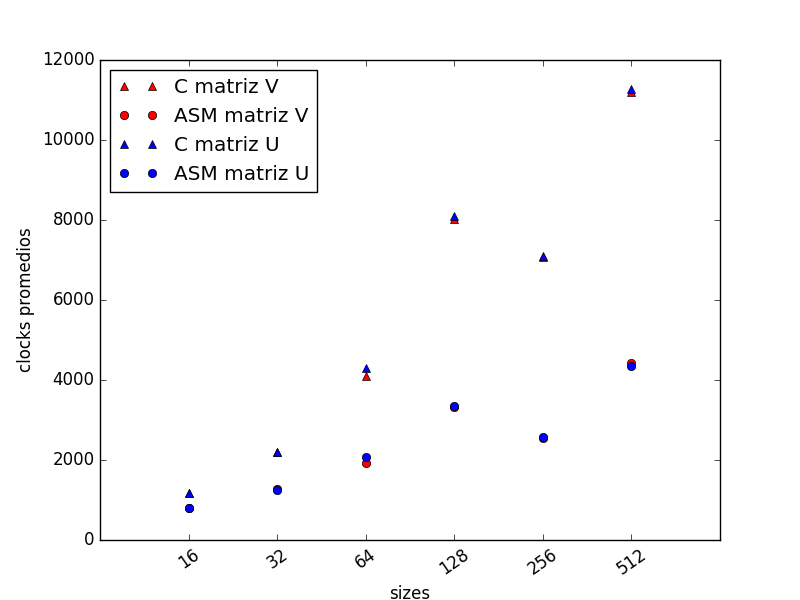
\includegraphics[width=.6\linewidth]{ClocksCYASMMAL.png}
  	\caption{ASM VS C solver$\_$set$\_$bnd con 200 iteraciones}
  	\label{fig:ASMU}
\end{figure}

\clearpage


\clearpage

\end{document}
